\documentclass[pdftex,12pt,letter]{article}
\usepackage[margin=0.75in]{geometry}
\usepackage{verbatim}
\usepackage{graphicx}
\usepackage{cite}
\usepackage{color}
\usepackage[binary-units=true]{siunitx}
\usepackage[pdftex,pdfpagelabels,bookmarks,hyperindex,hyperfigures]{hyperref}

\bibliographystyle{unsrt}

\newcommand{\fixme}[1]{\textbf{FIXME: #1}}    


\title{Unified Online/Offline Storage Buffer\\for Single-Phase ProtoDUNE}
\date{\today}
\author{B. Viren}

\begin{document}
\maketitle

\begin{abstract}
  The Single-Phase (SP) ProtoDUNE detector must provide for a local storage
  buffer sufficient for at least three days of data.  The note gives
  designs for this storage based on close unification between online
  and offline processes.
\end{abstract}

\tableofcontents

\pagebreak

\section{Overview}

This document describes a spectrum of possible designs for a unified
online/offline storage buffer for the Single-Phase (SP) ProtoDUNE
detector.  This buffer is required to potentially cache as much as
three days worth of nominal data acquisition, as required by CERN.
During nominal running it serves as a staging area for data transfer
to CERN EOS disk system.  This transfer is expected to be performed by
the Fermilab File Transfer System (F-FTS or just FTS).

The expected data rates are such that commodity hardware will present
a bottleneck unless the buffer maintains a parallel architecture.
Given that the DAQ itself is parallel in nature, these designs for the
buffer attempt to mesh with the design of the DAQ.  This tight
integration leads to an overall leaner system but will require close
attention by both online and offline members.

More than one design is considered as there are a few crucial
requirements that have come up which have strong impact on the design
and which can be satisfied in more than one way.  In particular, do we
require:

\begin{itemize}
\item sequential trigger numbers in a raw data file?
\item contiguous readout fragments for a given trigger in a raw data file?
\item the DAQ satisfy these two requirements or do we transfer them to the offline?
\end{itemize}

In the following sections, a review of our current understanding of
the SP data rates is given, then the DAQ is described at a high level.
Finally, a number of optional designs for a unified online/offline
buffer are described.

\section{Data Rates}

The ``protoDUNE/SP Data Scenarios'' spreadsheet
v5\footnote{\url{http://docs.dunescience.org:8080/cgi-bin/ShowDocument?docid=1086&version=5}}
describes three possible running conditions and estimates for their
resulting data volumes and rates and interpretations in terms of
network and disk bandwidth.  It also includes estimates for non-beam
trigger for acquiring additional cosmic-$\mu$ data.  Some highlights
of these estimates for the mid-range (so called ``Goldilocks'')
scenario are in Table~\ref{tab:goldi}.

\begin{table}[htbp]
  \centering
  \begin{tabular}[h]{l|r}
    Trigger rate & \SI{10}{\Hz} \\
    Spill time & \SI{4.8}{\second} \\
    Cycle time & \SI{16.8}{\second} \\
    Readout time & \SI{5}{\milli\second} \\
    \#APA & 3 \\
    \hline
    Readout & \SI{115}{\mega\byte} \\
    Compression & $\times$5 \\
    Instant rate & \SI{230}{\mega\byte\per\second} \\
    Average rate & \SI{66}{\mega\byte\per\second} \\
    \hline
    3-Day volume & \SI{17}{\tera\byte} \\
    \hline\hline
    cosmic-$\mu$ & $\times$2 \\
  \end{tabular}
  \caption{Parameters governing data rates and volumes for the ``Goldilocks'' (v5) scenario.  See text.}
  \label{tab:goldi}
\end{table}

The current assumption is that for every beam trigger one non-beam
trigger (cosmic-$\mu$ in the table) be acquired during the time when
the beam is not spilling.  This assumption represents a doubling of
the data rates and volumes presented in Table~\ref{tab:goldi}.  The
instant and average rates are those for when the beam is spilling or
if the rate is amortized over the entire beam cycle. 

At face value this data scenario is very modest but two things to
note.  First, even with these modest numbers some level of parallelism
is needed to sustain the expected bandwidth on commodity hardware
(Gbps network interfaces, \SI{50}{\mega\byte\per\second} disk).  The
second issue is that the scenario is based on uncertain parameters
which are known to lead to underestimates.  The scenario is expected
to grow substantially as they are better known.  In particular:

\begin{itemize}
\item A \SI{10}{\Hz} trigger rate is assumed although the beam can
  deliver hundreds of \si{\Hz} of particles.  
\item Trigger efficiency and purity is assumed to be 100\% meaning
  exactly 5M triggers are needed to satisfy the run plan.
\item It is assumed the SP detector will achieve a noise level no
  worse than MicroBooNE and thus can also achieve the associated
  compression factor of $\times5$.
\end{itemize}
One can imagine one or all of the following extreme problems might arise:
\begin{itemize}
\item The trigger rate goes to
\SI{50}{\Hz} in order to ``catch up'' with the run plan after some
delays
\item The triggering ends up being only 50\% pure requiring
  acquisition of 10M triggers.
\item The noise level achieved is closer to that of the 35t causing
  compression factor to fall to $\times 2$.
\end{itemize}
If all these extreme contingencies were to occur together their affect
on the buffer is estimated as in Table~\ref{tab:expansion}.
\begin{table}[htbp]
  \centering
  \begin{tabular}[h]{r|rl}
    volume & $\times10$ & \SI{3.3}{\peta\byte} total raw data \\
    \hline
    writes & $\times25$ & 13 Gbps, 65 parallel HDDs, \\
    \hline
    buffer & $\times25$ & \SI{850}{\tera\byte}, 3-days\\
  \end{tabular}
  \caption{Worse case scenarios where trigger rate, trigger selection and noise are such that they all increase the amount of data.}
  \label{tab:expansion}
\end{table}

As we better understand 35t and MicroBooNE data as well as the CERN
beam and its instrumentation it is expected these extremes will come
down in scale.  If we take them as is they represent a range of scale
of more than order of magnitude.  The buffer (and DAQ) designs should
scale across at least this range.  We must plan to implement a system
that is adequate for the ``worse reasonable case'' as the actual data
rates will not be known until SP begins commissioning.  Such concrete
planning and procurement must follow.  For this document we limit the
discussion to just the design.

\section{DAQ Throughput and Multiplicity}

This section describes how the DAQ is modeled in order to understand
its throughput and the node multiplicity.  The basic DAQ up to event
building is described and the model is applied to the nominal data
scenario.

\subsection{DAQ Model}

The ProtoDUNE SP DAQ is as an asynchronous, distributed and networked
data processing application.  At a high level of abstraction it can be
seen as a linear pipeline of functions $f_i$.  However, each function
$f_i$ has a number $N_i$ of instances or \textit{nodes} which run
independently and concurrently.  These nodes are arranged
topologically into a common \textit{layer}.  The sequential layers
then make up the pipeline.  One node may receive as input data from
one or more nodes in a prior layer and may send its output to nodes in
a subsequent layer.

The pipeline can also be considered a directed acyclic graph with
vertices identified with the functions and edges consisting of data
transfer paths.  Physically, a vertex are mapped to a service running
on computer host and an edge is mapped to a communication link.  The
layered topology makes the graph similar to but with functionality
different than that of an artificial neural network.

\begin{figure}[htbp]
  \centering
  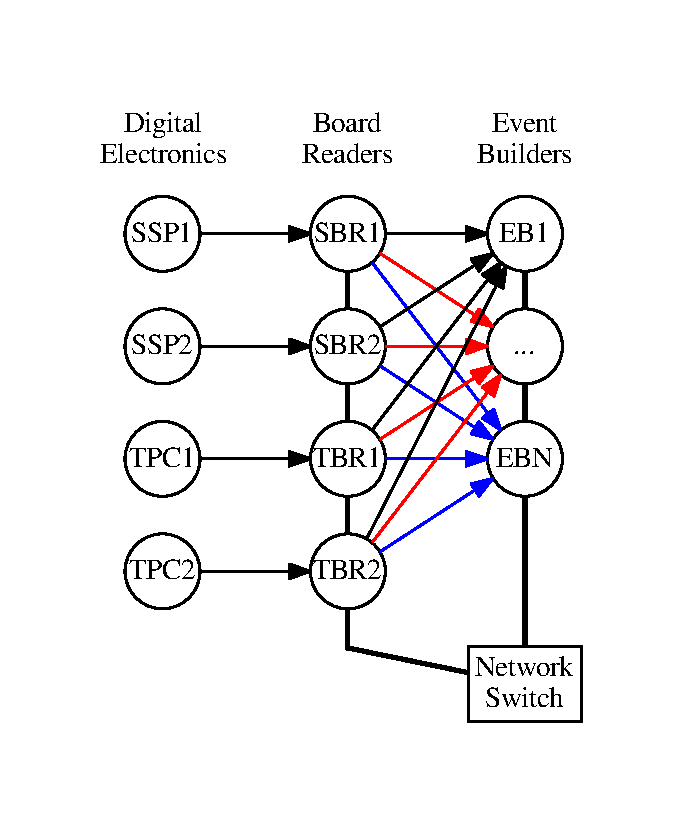
\includegraphics[width=0.5\textwidth]{upstream.pdf}
  \caption{Some fraction of the upstream portion of the DAQ.}
  \label{fig:upstream}
\end{figure}

The connectivity of a portion of the upstream part of the DAQ is
illustrated in a general way in Fig.~\ref{fig:upstream}.  A node in
the Digital Electronics (DE) layer provides the source of data for one
portion of the detector, either optical (SSP) or wire waveforms (TPC).
These fragments enter the DAQ via Board Readers (BR).  Each fragment
from a common trigger carries a common trigger number which is
indicated in the diagram by a colored arrow.  Based on that number,
fragments from the same trigger are sent to a common event builder
(EB) node for assembly.  In the figure, all fragments from a ``black
trigger'' is sent to EB1 and all fragments from a
``\textcolor{blue}{blue trigger}'' are sent to EBN.

The number of nodes in the BR layer is determined by channel
multiplicity of the detector electronics that are to be read out.
Given the nature of the DAQ application, there is freedom to choose
the multiplicities of the Event Builder and subsequent layers
discussed below.  The optimum choice is a balance of performance (more
nodes) and cost (fewer nodes).  For a given set of assumptions a
number of minimum requirements can be derived.  A single DAQ node is
modeled generally and independently from its function in terms of its:
\begin{itemize}
\item $B_{in}$,  input bandwidth 
\item $S_{in}$, input data size (per trigger)
\item $\tau$, processing time (per trigger)
\item $S_{out}$, output data size (per trigger)
\item $B_{out}$,  output bandwidth
\end{itemize}
These five terms imply a synchronous
processing model:
\begin{enumerate}
\item The node receives all its input data.
\item The node processes input to produce output.
\item The node sends all its output data.
\end{enumerate}
However, given suitable data structures and algorithms, a node may
begin sending output data while it is still receiving input data for
the same trigger.  This potential optimization is neglected in this
model.  Also ignored are effects due to fluctuations in data size and
processing time.  A final caveat is that the model so far does not
associate input and output to network interface hardware.  If multiple
nodes are hosted on a common computer, care is needed to properly
account for shared resources.

A few relations between these parameters are made obvious.
Data is conserved between sequential layers with node counts $N_i$
and $N_j$ respectively so that,
\begin{equation}
  \label{eq:dataconservation}
  N_i \times S_{i,out} = N_j \times S_{j,in}
\end{equation}
A \textit{maximum throughput} of a node can be defined as the maximum
number of triggers per second it can allow to pass.  It is defined by
its bottleneck throughput which is either due to input, processing
time or output:
\begin{equation}
  \label{eq:throughput}
  T_{max} = min(B_{in}/S_{in}, 1/\tau, B_{out}/S_{out})
\end{equation}
In order for any given layer $i$ with number $N_i$ nodes to not present a
bottleneck to the data flow its nodes must have a maximum throughput greater
than the detector trigger rate $R_{trig}$:
\begin{equation}
  \label{eq:minthroughput}
   T_{i,max} > R_{trig} / N_i
\end{equation}

The arrows in Fig.~\ref{fig:upstream} indicate logical data flow
between nodes.  Actual data flow between some layers, such as between
BR and EB nodes, is concentrated through a network switch.  In order
to not pose a bottleneck a switch between the two layers must pass a
bandwidth of
\begin{equation}
  \label{eq:switchbw}
  B_{switch,ij} > r_{trig} \times S_{i,out} =r_{trig} \times S_{j,in}
\end{equation}
where the two $S$ give equivalently the size of data corresponding to
a single trigger and which is passing out of layer $i$ and in to $j$.
Note that this inequality is independent from the number of nodes in
either layers.  The requirement is on the switch fabric and the
requirement on the per-port bandwidth is lower by a factor
$1/N_i$.



\subsection{An Example}

For the data scenario considered, we can require that 
the switch between BR and EB layers must provide at least
enough bandwidth to accommodate the nominal peak rate which occurs
during the spill.  This is \SI{230}{\mega\byte\per\second}
or just under 2~Gbps.  If transmission of beam trigger data is
averaged over the beam cycle and including non-beam triggering then
the minimum switch fabric bandwidth is relaxed to just above 1~Gbps.

For the EB layer to not present a bottleneck each term in the $\min$
function of Eq.~\ref{eq:throughput} must satisfy
Eq.~\ref{eq:minthroughput}.  Assuming no compression and a commodity
NIC providing 1~Gbps full-duplex the input and output bandwidth terms
indicate $N_{EB} \geq R_{trig}S_{evt}/B = 2$ in order to pass
\SI{230}{\mega\byte\per\sec}.  If this number of nodes is accepted it
places a requirement back on to the EB node to complete processing of
one trigger in
$\tau_{EB} \leq N_{EB}/R_{trig} = 200$~\si{\milli\second}.  If the
event building must take longer than this then it becomes the
bottleneck and either the process must be sped up or more nodes are
required.

\section{DAQ Options}

Starting at the EB layer of Fig.~\ref{fig:upstream} a number of
options are considered that extend the distributed DAQ to meet the
buffer while not creating a bottleneck.  They differ in trade offs of
node multiplicity and features.

\subsection{Immediate Write}

The simplest extension of the basic upstream DAQ configuration is to
add local disks and an instance of F-FTS to the computers hosting the
EB services.  This option is termed \textit{Immediate Write} and the salient
parts are illustrated for a single host in Fig.~\ref{fig:immediate}.

\begin{figure}[htbp]
  \centering
  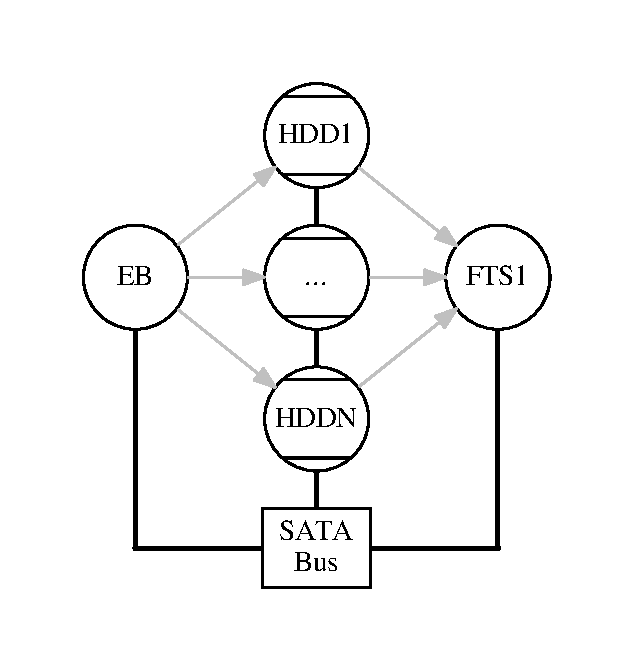
\includegraphics[width=5cm]{eb2ld.pdf}
  \caption{The \textit{Immediate Write} option to connect one EB to local
    buffer disk storage.}
  \label{fig:immediate}
\end{figure}

In this local context of a single host the same basic model can be
applied.  The ``nodes'' here include a process that writes the data to
a storage unit (HDD) and then makes this data available to F-FTS,
which also fits in to the model as a node.  At its simplest, this HDD
``process'' is nothing more than \texttt{write()} and \texttt{read()}
functions in EB and FTS, respectively.  However, FTS requires a
metadata file including a checksum and it is desirable to produce both
before the file is written to avoid extra HDD I/O.

The switch between the three layers in this case is the host SATA bus
which provides a greater bandwidth than the a commodity 1~Gbps NIC
(SATA III provides 6~Gbps).  Some modern HDD can sink or source 1~Gbps
but most can not do both simultaneously.  At least two HDD are assumed
in order to meet the more modest requirement of minimum HDD bandwidth
of \SI{50}{\mega\byte\per\second} and to avoid simultaneous reads and
writes on the same media.

While this design is simple and requires only minimal extra hardware
it has the following consequences:  

\begin{itemize}
\item Interlaced triggers.  The events from the EB node that are saved
  to disk will not be sequential because the EB does not receive
  sequential triggers from the upstream BRs.  While one EB is building
  an event from trigger $i$ another EB node will be building trigger
  $i+1$.  See \textit{Sorted} and \textit{Preprocessed} options for an
  alternative.
\item Tight coupling.  The EB processing and FTS-related processing
  (metadata and checksumming) may lead to CPU contention.  Placing
  three functions (EB, storage, FTS) on one host means the failure of
  any one likely means the failure of all.  See \textit{Decoupled Write}
  option for an alternative.
\end{itemize}

\subsection{Sorted}

It is convenient to have sequential triggers in raw data files but it
is becoming less and less required as experiments take higher rate
data.  A naive approach to providing sorted raw data files is to
concentrate all strings into one point.  This requires a massive
monolithic computing element and this idea is discarded.

Another approach is to use some intelligent upstream routing to
collate built events into sequential order.  This requires an extra
layer of \textit{Event Sorter} (ES) nodes.  These nodes must maintain
a buffer in memory of some number of events which can be as many as
what an entire file holds.  However, this load can be spread across
multiple ES nodes so that multiple events in multiple files need not
be cached in a single memory system.  As detailed next, the resulting
files will themselves still be interlaced but this out-of-order issue
is erased through the use of a file catalog.

The ES nodes work in partnership with the EB nodes.  The EB nodes are
extended to accept a configuration parameter which is the number of
triggers in to be saved in each file.  They further have a static
function which maps this configuration parameter and the current
trigger number to the address of an ES node.  An obvious example is
that to determine the ES index via integer division and modulus.
Then, for $N_{ES}$ nodes and each file holding $N_{file}$ triggers
an EB node determines which ES to send its data by $(i/N_{file})\%N_{ES}$.

For writing to buffer the ES node can reside on host as the EB node in
\textit{Immediate Write} or in \textit{Decoupled Write}

\subsection{Decoupled Write}

This variant extends \textit{Immediate Write} to move the EB (or ES)
node off of the same host as the storage.  This requires a new service
to accept data from the EB (or ES) node and write it to disk.  This
new service can be based on artDAQ which makes it part of the DAQ
proper.  Alternatively, it can use another protocol such as Xrootd in
which case the EB (or ES) must be developed to speak this protocol.
If additional processing is required (such as metadata file production
and checksumming) as the data is written then an artDAQ implementation
for this node is likely best.

\subsection{Preprocessed}

If the requirement of sequential triggers is required then it can be
accomplished in an offline context.  The essential idea is that an
offline process close to the source of the interlaced data files reads
in multiple stream, performs deinterlacing and writes out sequential
files.  This will be a highly I/O bound and data intensive job.

It does open an opportunity to add a modest amount of processing in
order to reap a reduction in the output data volume.  The resulting
files can then be sent to distributed processing without incurring I/O
penalties.  This additional processing might be the following:

\begin{enumerate}
\item DAQ write interlaced events from EB (or even interlaced fragments directly from BR)
\item Archive interlaced files via F-FTS
\item Infrequently preprocess the as:
  \begin{enumerate}
  \item Read N interlaced files as parallel streams and deinterlace.
  \item Apply software noise removal.
  \item Apply detector response deconvolution.
  \item Apply thresholding saving only signals above.
  \item Write and archive a single, much smaller file.
  \end{enumerate}
\item Production reconstruction processing on this reduced file.
\end{enumerate}
This processing requires discrete Fourier transforms and their inverse
to be run on each raw FADC waveform.  The full reconstruction steps
are estimated to require $5-10\times$ more CPU than these steps.  The
size reduction needs study but is roughly estimated to be
$10-100\times$.  Even in the absence of interlacing, this is a very
advantageous approach.  

\end{document}

%%% Local Variables:
%%% mode: latex
%%% TeX-master: t
%%% End:
